\section{Data collection}
Although one may have the intuition that the texture patterns of some
images are easier to be re-synthesized than those of other images,
quantifying this intuition has not been addressed. In order to learn
image synthesizability, we collectd a database and annotated it in
terms of synthesizability. The dataset contains $32,000$ texture
images, with $2000$ delibratedly collected general textures of a
variety of kinds such as stochastic, repetitive, irregular, cluttered
scenes, and $30,000$ texture images retrieved by searching in Google
with $30$ keywords, each for $1000$ images. The keywords we used are:
painting texture, flower texture, grass texture, concrete texture,
wood texture, woven texture, glass texture, water texture, stone
texture, plastic texture, fabric texture, leather texture, metal
texture, paper texture, brick texture, marble texture, fur texture,
urban texture, noodle texture, wall texture, regular
texture, irregular texture, stochastic texture, lined texture,
circular texture, flowing texture, repetitive texture, speckled
texture, wrinkled texture, and cracked texture.

For annotation, we characterize synthesizability as the goodness of
synthesized image. A good synthesized image should be as similar as
possible to the input example and should not have visible artifacts
such as seams, blocks and misfitting edges, and should not have
visible repetition of same image structures. Since no ETS method
performs better than others on all kinds of textures -- each of them
performs well for certain texture examples, and poorly for others.  We
employed five ETS methods of different flavourings, and labeled the
`best' synthesized result. The philosophy of synthesizability is how
well the underlying visual patterns can be re-synthesized by learning
on a single example, no matter what learning methods we use.  Five
methods of different flavourings were employed, and they are: image
quilting~\cite{Efros:sig2001}, graph-cut based
method~\cite{Kwatra:2003}, clique-based MRF~\cite{Zalesny05},
wavelet-based paramatric method~\cite{Portilla:2000:IJCV}, and random
phase synthesis~\cite{random:phase}. While futher study will be needed
when more powerful example-based texture synthesis (ETS) methods are
proposed, this dataset consistitute an initial benchmark.  The
goodness is divided into three levels: good, acceptable, and bad,
corresponding to $1$, $0.5$ and $0$ of image synthesizability.
Fig.~\ref{fig:dataset} shows several examples of the annotation.  The
dataset will be publically available upon the acceptance of the paper.

\begin{figure} [!t]
  \centering
   $ \begin{array}{cccc}
\hspace{-1.5mm}
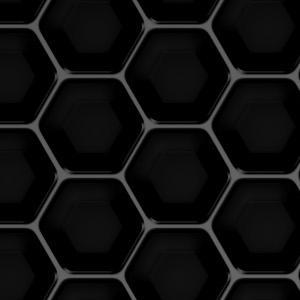
\includegraphics[width=0.23\linewidth]{./figs/dataset/87.jpg} & 
\hspace{-3mm}
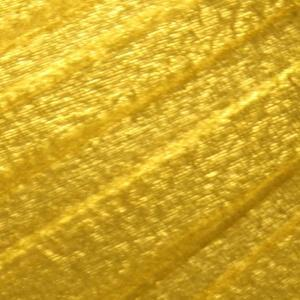
\includegraphics[width=0.23\linewidth]{./figs/dataset/76.jpg} & 
\hspace{-3mm}
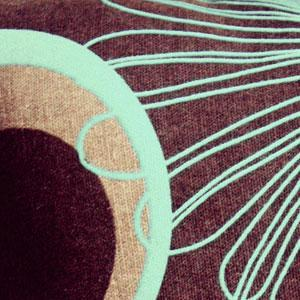
\includegraphics[width=0.23\linewidth]{./figs/dataset/43.jpg} \\ 
\hspace{-1.5mm}
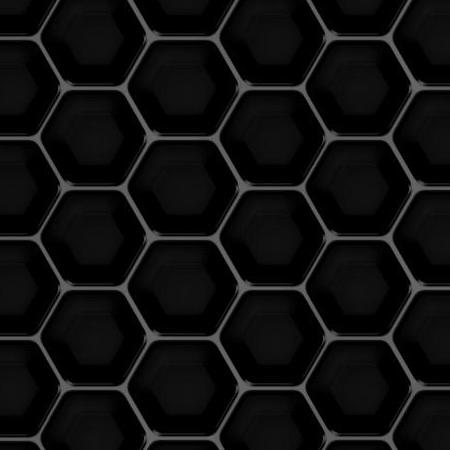
\includegraphics[width=0.33\linewidth]{./figs/dataset/87syn.jpg} & 
\hspace{-3mm}
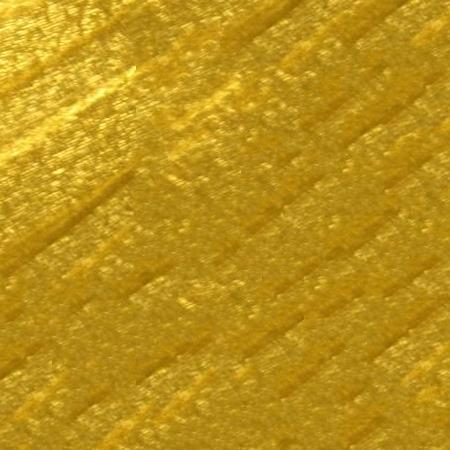
\includegraphics[width=0.33\linewidth]{./figs/dataset/76syn.jpg} & 
\hspace{-3mm}
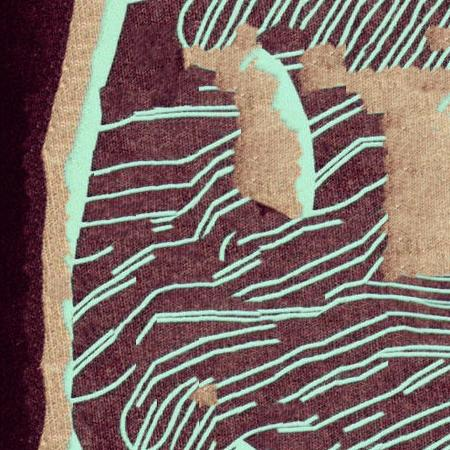
\includegraphics[width=0.33\linewidth]{./figs/dataset/43syn.jpg} \\ 
\scriptsize{\text{Good (1)}} & \scriptsize{\text{Acceptable (0.5)}} & \scriptsize{\text{Bad (0)}}  \\

\end{array}$
\caption{Three texture examples from our dataset with their
  annotations of synthesizability, where top are texture examplars and
  bottom show corresponding synthesized ones. }
  \label{fig:dataset}
\end{figure}

